% Generated preview. Edit papers/sprint-risk/sections and rebuild.
\documentclass[11pt,a4paper]{article}
% Source: preamble.tex
\usepackage[margin=24mm]{geometry}
\usepackage[T1]{fontenc}
\usepackage[utf8]{inputenc}
\usepackage{lmodern}
\usepackage{amsmath,amssymb}
\usepackage{booktabs,longtable,array,calc}
\usepackage{graphicx}
\usepackage{xurl}
\usepackage{hyperref}
\usepackage{pgfplots}
\usepgfplotslibrary{groupplots}
\pgfplotsset{compat=1.18}
\hypersetup{colorlinks=true,linkcolor=blue!50!black,citecolor=blue!50!black,urlcolor=blue!50!black}
\providecommand{\tightlist}{\setlength{\itemsep}{0pt}\setlength{\parskip}{0pt}}
\setlength{\emergencystretch}{3em}
\setlength{\parskip}{0.3em}
\makeatletter
\setlength{\@fptop}{0pt}
\setlength{\@fpsep}{12pt}
\setlength{\@fpbot}{0pt plus 1fil}
\makeatother
\title{Early Warning of Recorded Sprint Non-Completion:\\Execution Histories, Calibration, and Alert Budgets}
\author{Anonymous manuscript draft}
\date{8 October 2026}

\begin{document}
\maketitle
% Source: sections/00_abstract.tex
\begin{abstract}
Issue trackers contain execution histories that may support early identification of work unlikely to finish within a sprint. However, retrospective evaluations can confuse forecasting unfinished work with recognizing work already completed, and percentage-based alert budgets can behave unexpectedly in small cohorts. We conduct an archival study using TAWOS v1.1, reconstructing 28,746 issue--sprint commitments from timestamped membership changes. Of these, 22,147 have assessable outcomes, yielding 88,588 snapshots at four sprint landmarks. Fourteen projects, containing 18,322 labeled instances, meet the evaluation criteria. We compare six methods using chronological within-project splits and leave-one-project-out evaluation, with validation-only probability recalibration. At the midpoint, dynamic CatBoost increases sprint-macro recall from 44.46\% to 53.36\% over matched static CatBoost on temporal tests, a difference of 8.90 percentage points (95\% paired-bootstrap interval: 6.38--11.70). However, the difference falls to 2.59 points when evaluating only issues still open. Rounding a nominal 20\% budget upward produces a temporal mean sprint-level allocation of 41.54\%; strict downward rounding reduces dynamic recall to 18.20\%, while retaining a positive difference over the static model. Recalibration improves temporal Brier score but not cross-project Brier score. A simple execution-state rule is competitive, and its temporal recall difference from dynamic CatBoost is inconclusive. These findings support the predictive value of recorded execution histories while showing that eligibility, integer capacity, strong baselines, and calibration transfer materially affect practical conclusions. Outcomes are tracker-state proxies under archived sprint-date assumptions, not independently verified delivery or causal intervention outcomes.

\end{abstract}
\noindent\textbf{Keywords:} empirical software engineering; sprint outcome prediction; issue tracking; predictive process monitoring; probability calibration; budget-constrained alerting.

% Source: sections/01_introduction.tex
\section{Introduction}\label{introduction}

Sprint monitoring involves identifying work that may remain unfinished when a planning interval ends. Issue trackers record status transitions, sprint assignments, and other attribute changes that provide a partial trace of execution. A useful warning system must prioritize a limited number of issues at a time when action is still possible. Predictive accuracy alone is therefore insufficient: predictions must be available at the decision time, probabilities must be interpreted cautiously, and alerts must respect an explicit handling capacity.

Three evaluation choices are especially consequential. First, tracker attributes observed at data collection can differ from those available at prediction time. Tu et al.~examine this problem in issue-tracking research \cite{tu2018careful}. Second, a midpoint classifier may distinguish already-completed issues from all other issues without providing comparable improvement on work that remains open. Third, an apparently uniform percentage budget can allocate very different effective fractions across sprints when integer rounding is required.

We investigate these issues through an archival replay study. Our target is \textbf{recorded non-completion at the archived sprint end date}, rather than an independently verified failure to deliver business value. We use TAWOS v1.1 \cite{tawosi2022tawos,tawosv11} and construct issue--sprint instances supported by timestamped membership evidence. We compare information fixed at sprint start against additional execution history available at standardized landmarks. We evaluate chronological transfer, project transfer, calibration, and both single-landmark and cumulative alert policies.

The study makes three empirical contributions:

\begin{enumerate}
\def\labelenumi{\arabic{enumi}.}
\tightlist
\item
  A reproducible procedure for cohort reconstruction, outcome assessment, prefix feature extraction, and label-availability-aware splitting, with explicit exclusion and provenance artifacts.
\item
  Evidence about the incremental value of execution histories, including controls for already-completed work, scope changes, recurring issues, and a strong rule-based comparator.
\item
  An analysis of how integer budget allocation and calibration transfer change the interpretation of early-warning performance.
\end{enumerate}

We do not propose a new learning algorithm or claim state-of-the-art performance. The contribution is an auditable evaluation of a specific decision setting, including results that limit the case for deploying a learned model.

% Source: sections/02_related_work.tex
\section{Background and Related Work}\label{background-and-related-work}

\subsection{Agile issue datasets and effort estimation}\label{agile-issue-datasets-and-effort-estimation}

TAWOS provides descriptive attributes and change histories from Agile open-source projects \cite{tawosi2022tawos,tawosv11}. Its breadth enables questions beyond effort estimation, but a current issue--sprint relation does not itself establish membership at the beginning of a historical sprint. Version identification is also necessary: the introductory paper and the v1.1 repository describe different project counts. We use the latter snapshot and do not combine their populations.

Effort estimation and sprint non-completion prediction have different targets. For example, Bui et al.~study an LLM-based multi-agent approach to Agile effort estimation \cite{bui2025agents}. Predicting an effort estimate does not directly answer whether an issue will be in a recorded terminal state by a sprint endpoint. Consequently, effort-estimation performance measures cannot be treated as comparable baselines for recall under an alert budget.

\subsection{Outcome-oriented predictive monitoring}\label{outcome-oriented-predictive-monitoring}

Outcome-oriented predictive process monitoring predicts a case outcome from a partial execution trace. Teinemaa et al.~organize and benchmark methods for this setting \cite{teinemaa2019outcome}. Our study adopts the prefix-to-outcome perspective, but defines cases as issue--sprint instances with a shared sprint endpoint and a cohort fixed at sprint start. Multiple instances can arise from the same issue across different sprints. Membership changes and reopened issues therefore require handling beyond an issue-level snapshot classifier.

\subsection{Temporal validity, learners, and calibration}\label{temporal-validity-learners-and-calibration}

Time-related misuse of issue-tracking data motivates reconstructing what the recorded history supports at each landmark \cite{tu2018careful}. CatBoost is a tabular learner supporting categorical features \cite{prokhorenkova2018catboost}; we use it as a matched learner for static and dynamic inputs, not as an established best method for this task. Probability calibration is a separate estimation step and must use data outside the base learner's fitting sample \cite{sklearncalibration}. Recalibration learned from other projects may nevertheless fail to transfer to a held-out project.

This related-work discussion is a targeted positioning of the experiment, not a systematic literature review or evidence that no previous study has considered an equivalent task.

% Source: sections/03_research_questions.tex
\section{Research Questions and Target}\label{research-questions-and-target}

\textbf{RQ1 --- Incremental information:} At the midpoint of a sprint, does observed execution history improve budget-constrained identification of recorded non-completion over information available at sprint start?

\textbf{RQ2 --- Transfer:} How does this comparison behave on later sprints within a project and on projects excluded from training and calibration?

\textbf{RQ3 --- Decision conditions:} How do active-work eligibility, integer alert budgets, probability recalibration, and cumulative alerting affect the interpretation of model performance?

Let \(s\) denote a sprint, \(i\) an issue, and \(t_{0s}\) and \(t_{1s}\) its archived start and end dates. For landmark \(\lambda\in\{0,0.25,0.50,0.75\}\), define

\[
t_{s,\lambda}=t_{0s}+\lambda(t_{1s}-t_{0s}).
\]

The target is

\[
Y_{is}=\mathbb{1}\{S_i(t_{1s})\notin\mathcal D\},
\qquad \mathcal D=\{\text{Done, Resolved, Closed, Complete}\},
\]

where \(S_i(t)\) is the last assessable recorded status at or before \(t\), with case-insensitive matching. Unknown or ambiguous outcomes are not assigned to either class. The estimand is conditional on the subset for which membership and outcome can be assessed under the audit rules.

The primary hypothesis, fixed locally before model fitting and test evaluation, concerns

\[
\Delta_T=\frac{1}{|\mathcal S_+|}\sum_{s\in\mathcal S_+}
\left[R_s^{\mathrm{dynamic}}(0.50,0.20)
-R_s^{\mathrm{static}}(0.50,0.20)\right],
\]

where \(\mathcal S_+\) comprises temporal test sprints with at least one positive outcome and \(R_s\) is recall under the registered upward-rounded budget. Evidence supports H1 when \(\Delta_T>0\) and its 95\% paired-bootstrap interval excludes zero. The cross-project contrast uses equal project weights and is secondary. The protocol was recorded in local Git, \textbf{not publicly preregistered with an external registry}.

% Source: sections/04_data.tex
\section{Data and Historical Reconstruction}\label{data-and-historical-reconstruction}

\subsection{Source and cohort flow}\label{source-and-cohort-flow}

TAWOS v1.1 contains 458,232 issues from 39 projects, 4,594 sprint records, and 9,253,419 changelog entries \cite{tawosv11}. We retain closed sprints with valid start/end dates, a positive duration between 1 and 60 days, and a start year of at least 2000. These are operational data-quality criteria, not claims about ideal sprint duration.

Sprint changelog values represent sets of Jira sprint identifiers. We map them by \texttt{(project\_\allowbreak{}id,\ jiraid)}, rather than by the dataset's internal sprint primary key. An issue belongs to a reconstructed start cohort when it was created by the archived start time and the last membership event at or before that time contains the target sprint. Issues added later are excluded from that sprint's start cohort. References without a corresponding sprint record are logged rather than guessed.

{\def\LTcaptype{table}
% Source: tables/01_cohort.tex
\begin{table}[htbp]
\centering\footnotesize\setlength{\tabcolsep}{4pt}
\caption{Source, reconstructed, and evaluation populations. The source row counts issues, not issue--sprint instances.}\label{tab:01_cohort}
\begin{tabular}{@{}lrrr@{}}
\toprule
Population / partition & Projects & Sprints & Issues / instances \\
\midrule
Source snapshot & 39 & 4,594 & 458,232 issues \\
Reconstructed membership-supported cohort & --- & --- & 28,746 \\
Cohort with assessable outcomes & --- & 2,555 & 22,147 \\
Eligible evaluation population & 14 & 1,962 & 18,322 \\
Temporal training & 14 & 1,165 & 11,500 \\
Temporal validation & 14 & 383 & 3,401 \\
Temporal test & 14 & 397 & 3,293 \\
Purged temporal boundary instances & --- & 17 & 128 \\
\bottomrule
\end{tabular}
\end{table}

}

Outcome coverage is 77.04\% of membership-supported instances; 6,599 outcomes remain unassessable under the rules. Four landmarks yield 88,588 snapshots across the labeled reconstructed population. Table 1's temporal partitions concern the 14 eligible projects, not all labeled projects.

\subsection{Outcomes, scope changes, and audit rules}\label{outcomes-scope-changes-and-audit-rules}

We replay recorded status transitions forward. Before the first observed status transition, status is \texttt{unknown}; neither the final issue snapshot nor a future event's prior-value field supplies a historical prediction feature. Ambiguous status names, including Accepted, Implemented, Deployed, Released variants, and WAD, are excluded from the primary outcome definition.

We identify inconsistent consecutive membership or status records. A contradiction between an earlier event's new value and a later event's prior value indicates missing or inconsistent history. These checks can identify uncertain intervals and lead to membership exclusion or unassessable outcomes. They are retrospective data-quality checks, not prediction features. Quality filtering can therefore condition the evaluated population on later evidence, a limitation distinct from feature timestamp leakage.

An issue removed after sprint start remains in its start cohort. Reopened issues are labeled by their recorded state at the endpoint: reopening before the end can change the outcome, whereas reopening after the end does not. Cancellation-related and removal flags support sensitivity analysis; the main label still follows the terminal-state rule. A terminal record is a proxy and does not establish that the intended functionality was delivered.

We independently check 765 sampled instances from the eligible projects using SQL queries for membership and endpoint status, including both outcome classes and scope changes. Where available, the prior-value field of a later status event corroborates the endpoint assessment. This verifies consistency between the replay and the source records; it is not a human workflow audit or inter-rater agreement study.

\subsection{Features and temporal integrity}\label{features-and-temporal-integrity}

Static features are fixed at \(t_{0s}\). Dynamic inputs add observations through \(t_{s,\lambda}\). Both use the following groups:

{\def\LTcaptype{table}
% Source: tables/feature_groups.tex
\begin{table}[htbp]
\centering\footnotesize\setlength{\tabcolsep}{4pt}
\begin{tabular}{@{}p{0.20\linewidth}p{0.74\linewidth}@{}}
\toprule
Group & Recorded information \\
\midrule
Timing & Issue age, archived sprint duration, time since the latest selected event \\
Execution state & Last observed status, terminal-state indicator, status-observed indicator, time since the latest status change \\
Prefix activity & Status transition count, selected-field event counts, events since sprint start, assignee/priority/estimate change counts \\
Attributes & Priority, issue type, and story-point value when supported by prior change events \\
Cohort context & Start-cohort size and fraction in a recorded terminal state at the corresponding landmark \\
\bottomrule
\end{tabular}
\end{table}

}

Selected-field activity covers Sprint, status, resolution, priority, issuetype, assignee, and Story Points; it does not represent all tracker activity or comments. Missing categorical attributes are \texttt{unknown}. We do not substitute final attribute values for initial values lacking timestamped support. This conservative choice limits coverage of the static information that a real team may actually know.

Cohort aggregates are computed before excluding unassessable outcomes, preventing outcome availability from changing the progress features of retained instances. Issue, project, sprint, and user identifiers are not model features. Text, final resolution fields, future changes, and full-lifetime effort totals are excluded. Provenance timestamps are audit fields, not predictors.

Automated checks verify unique issue--sprint--landmark keys, consistent labels across landmarks, prefix timestamps not exceeding the prediction time, and correct cohort aggregation. Tests also verify that modifying or deleting future events does not change issue-prefix features and that changing future labels does not alter cohort aggregates. These checks establish implementation invariants under the archived-date assumptions; they do not prove that archived sprint dates were unchanged throughout execution.

% Source: sections/05_methods.tex
\section{Experimental Design}\label{experimental-design}

\subsection{Eligibility and splits}\label{eligibility-and-splits}

Projects require at least 50 labeled-cohort sprints, 200 labeled instances, and 30 instances per outcome class. Temporal evaluation additionally requires at least ten test sprints, ten instances per class in training, and five per class in validation and test. Eligibility is determined before observing predictive test performance.

Within each eligible project, sprints are ordered by start date and divided approximately 60/20/20 into training, validation, and test, with identical start timestamps assigned together. Training sprints ending at or after the validation boundary are purged; validation sprints ending at or after the test boundary are likewise purged. This ensures that fitting and recalibration do not require endpoint labels unavailable at the next partition's beginning. Temporal learners are fitted separately per project. All landmarks of an issue--sprint instance retain the same partition.

For cross-project evaluation, each of the 14 projects is held out once. Two of the other 13 projects are selected for validation using the fixed random seed, leaving eleven for training. Neither fitting nor recalibration uses the held-out project's data. This is archival project transfer, not a globally chronological simulation of deployment across organizations.

The same issue can appear in successive sprints. Identifiers are not predictors, and a sensitivity analysis excludes temporal test issue identifiers previously seen in training. This does not remove all dependence between instances or between projects sharing a repository.

\subsection{Methods}\label{methods}

We evaluate six methods:

\begin{enumerate}
\def\labelenumi{\arabic{enumi}.}
\tightlist
\item
  \textbf{Frequency:} the training-set non-completion proportion, constant within an evaluation fold before recalibration.
\item
  \textbf{Execution-state rule:} a terminal-state score of 0.01; otherwise \(\operatorname{clip}(0.5+0.02d+0.1u,0.01,0.99)\), where \(d\) is days since the latest selected event and \(u\) indicates unknown status. This is a fixed heuristic, not an optimized business rule.
\item
  \textbf{Static logistic regression:} start-time inputs, training-only numerical imputation/scaling and categorical one-hot encoding, inverse regularization strength \(C=1\), and up to 2,000 iterations.
\item
  \textbf{Static CatBoost:} start-time inputs and cohort size.
\item
  \textbf{Dynamic CatBoost:} static inputs plus current prefix information and cohort aggregates.
\item
  \textbf{Dynamic CatBoost without cohort context:} the dynamic feature set with cohort-related variables removed, including cohort size and both start/current aggregate fractions.
\end{enumerate}

The CatBoost methods use 400 trees, depth 5, learning rate 0.05, L2 parameter 5, and seed 20261008. They share the same configuration so that the principal comparison examines input information rather than different learner families. Numerical missing values use CatBoost's native handling. No oversampling or class weighting is applied. These are fixed configurations, not an exhaustive hyperparameter search. The zero-percent landmark is an information control: adding duplicate encodings at that landmark adds no future execution observations, although fitting can still differ.

\subsection{Probability recalibration}\label{probability-recalibration}

For every method and landmark, the base learner is fitted on training data only. A validation-only logistic recalibrator estimates

\[
\widehat p_{\mathrm{cal}}=\sigma\!\left(a+b\operatorname{logit}(\operatorname{clip}(\widehat p,10^{-6},1-10^{-6}))\right).
\]

The recalibrator uses \(C=10^6\) and is not constrained to positive slope. If validation lacks at least five observations in each class, the identity mapping is used. Raw and recalibrated scores are retained. In the midpoint primary contrasts, raw and recalibrated ranking produce identical differences; the conclusions therefore do not depend on an inverse midpoint calibrator. Test-set calibration slope/intercept are diagnostic fits only and are not applied back to predictions. Separately identifiable slope/intercept are not reported for constant scores.

\subsection{Metrics, budgets, and uncertainty}\label{metrics-budgets-and-uncertainty}

For an evaluable cohort of \(n_s\) issues, the registered primary allocation is \(K_s^{\uparrow}(q)=\lceil qn_s\rceil\). Issues are ranked by risk with a deterministic, label-independent issue--sprint hash for ties. Sprint recall is \(TP_s/P_s\) when \(P_s>0\); otherwise it is undefined and excluded from the recall mean. Such sprints remain in false-alert and applicable precision summaries. We also evaluate \(K_s^{\downarrow}(q)=\lfloor qn_s\rfloor\), which enforces a strict fractional cap but assigns no alerts to small cohorts. Budgets of 10\%, 20\%, and 30\% are evaluated.

Temporal primary results give equal weight to test sprints with positive outcomes. Cross-project primary comparisons give equal weight to projects after averaging their sprint recalls. We distinguish these from pooled issue-level recall and precision, and report realized budget both as the mean sprint fraction and as total alerts divided by total issues.

Additional probability measures are average precision (AP, not trapezoidal PR area), Brier score, reliability curves with ten fixed bins, and diagnostic calibration slope/intercept. Brier measures probability quality jointly with discrimination; a lower value alone does not establish improved calibration. Paired bootstrap intervals use 2,000 resamples of sprints for temporal comparisons and projects for cross-project comparisons. Landmarks are analyzed separately rather than treated as independent observations from the same instance.

Prespecified sensitivity analyses consider open issues only, strict budget rounding, exclusion of cancellation/removal cases, unseen issue identifiers, and an alternative Closed-only outcome. Closed-only rescoring does not retrain the model for the alternate target. Raw-ranking and project-weighted temporal checks were recorded before computing test metrics. Comparisons against the rule and ablation, and paired cumulative-policy contrasts, were added after viewing the primary results and are explicitly exploratory. We do not adjust those supplementary intervals for multiple comparisons.

\subsection{Cumulative alert replay}\label{cumulative-alert-replay}

At 25\%, 50\%, and 75\%, we allow cumulative quotas of \(\lceil K_s/3\rceil\), \(\lceil2K_s/3\rceil\), and \(K_s\), respectively, where \(K_s=\lceil0.2n_s\rceil\) is the total sprint cap. Previously alerted issues and issues currently recorded as Done are ineligible for another alert. Unused capacity can carry forward. We measure recall, false alerts, and the mean lead time of true alerts within each sprint, averaged over sprints with true alerts. Even the static ranking baseline uses current recorded Done status for this common eligibility filter; cumulative-policy comparisons therefore concern operational ranking policies, not purely static information alone.

% Source: sections/06_results.tex
\section{Results}\label{results}

\subsection{Execution history improves midpoint ranking over static inputs}\label{execution-history-improves-midpoint-ranking-over-static-inputs}

{\def\LTcaptype{table}
% Source: tables/02_performance.tex
\begin{table}[htbp]
\centering\footnotesize\setlength{\tabcolsep}{4pt}
\caption{Midpoint results under upward-rounded nominal 20\% budgets. Temporal recall and precision are sprint-macro; cross-project recall and precision are project-macro. False alerts are mean counts per sprint.}\label{tab:02_performance}
\begin{tabular}{@{}lrrrrrr@{}}
\toprule
Method & \shortstack{Temporal\\recall (\%)} & \shortstack{Temporal\\precision (\%)} & \shortstack{Temporal\\false alerts} & \shortstack{Cross-project\\recall (\%)} & \shortstack{Cross-project\\precision (\%)} & \shortstack{Cross-project\\false alerts} \\
\midrule
Frequency & 36.25 & 55.43 & 0.927 & 34.13 & 46.97 & 1.210 \\
Execution-state rule & 51.23 & 72.28 & 0.486 & 49.69 & 62.50 & 0.801 \\
Static logistic regression & 44.99 & 66.11 & 0.630 & 43.60 & 57.26 & 0.934 \\
Static CatBoost & 44.46 & 66.45 & 0.617 & 43.56 & 57.03 & 0.907 \\
Dynamic CatBoost & 53.36 & 75.32 & 0.423 & 53.52 & 67.08 & 0.646 \\
Dynamic w/o cohort & 54.23 & 75.28 & 0.416 & 52.80 & 66.49 & 0.659 \\
\bottomrule
\end{tabular}
\end{table}

}

The temporal dynamic--static difference is 8.90 percentage points (95\% CI: 6.38--11.70), supporting the locally fixed H1. The interval uses 336 positive-outcome sprints among the 397 temporal test sprints. Dynamic CatBoost finds 682 of 1,883 positive instances using 850 alerts, versus 605 for static CatBoost using the same allocation. Pooled precision increases from 71.18\% to 80.24\%, with false alerts decreasing from 245 to 168.

The cross-project project-macro difference is 9.96 points (CI: 7.53--12.82; 14 projects). Mean project-level differences are positive for all 14 projects in both evaluation settings, but this is not a claim of project-specific statistical significance. At the zero-percent control landmark, the differences are only 0.66 points temporal and 0.67 cross-project, and both intervals include zero.

% Source: figures/fig_projects.tex
\begin{figure}[htbp]
\centering
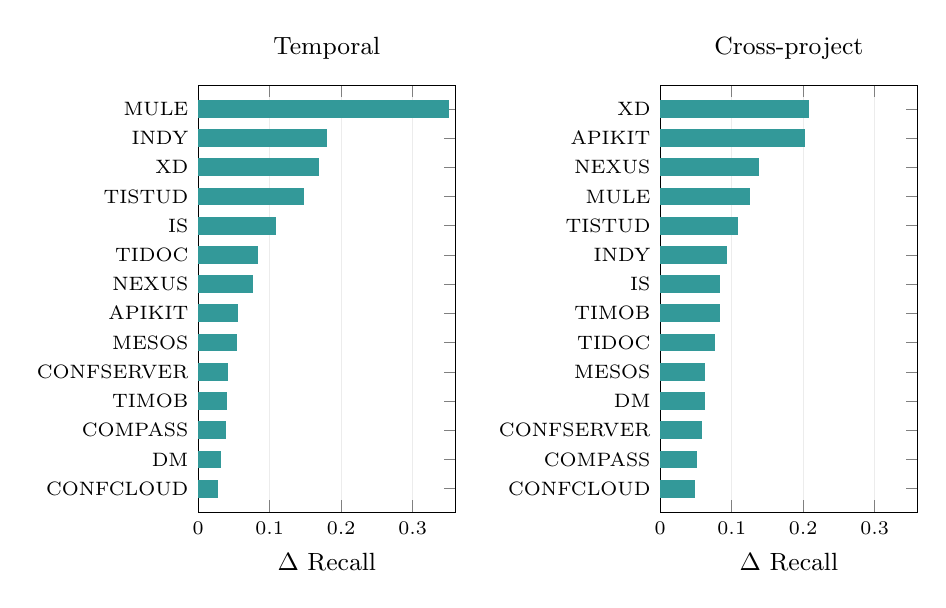
\begin{tikzpicture}
\begin{groupplot}[group style={group size=2 by 1,horizontal sep=2.6cm},width=0.40\textwidth,height=7cm,xmin=0,xmax=0.36,ymin=-0.8,ymax=13.8,xlabel={$\Delta$ Recall},tick label style={font=\scriptsize},label style={font=\small},title style={font=\small},xmajorgrids,grid style={gray!15}]
\nextgroupplot[title={Temporal},ytick={0,1,2,3,4,5,6,7,8,9,10,11,12,13},yticklabels={CONFCLOUD,DM,COMPASS,TIMOB,CONFSERVER,MESOS,APIKIT,NEXUS,TIDOC,IS,TISTUD,XD,INDY,MULE}]
\addplot[xbar,bar width=6pt,fill=teal!80,draw=teal!80] coordinates {(0.02631579,0) (0.03167901,1) (0.03846154,2) (0.03914169,3) (0.04151515,4) (0.05396825,5) (0.05555556,6) (0.07575758,7) (0.08333333,8) (0.10839161,9) (0.14705882,10) (0.16818182,11) (0.17948718,12) (0.35000000,13)};
\nextgroupplot[title={Cross-project},ytick={0,1,2,3,4,5,6,7,8,9,10,11,12,13},yticklabels={CONFCLOUD,COMPASS,CONFSERVER,DM,MESOS,TIDOC,TIMOB,IS,INDY,TISTUD,MULE,NEXUS,APIKIT,XD}]
\addplot[xbar,bar width=6pt,fill=teal!80,draw=teal!80] coordinates {(0.04829545,0) (0.05098336,1) (0.05806932,2) (0.06121430,3) (0.06230468,4) (0.07600151,5) (0.08221298,6) (0.08305195,7) (0.09308188,8) (0.10803571,9) (0.12455345,10) (0.13802083,11) (0.20119048,12) (0.20714200,13)};
\end{groupplot}
\end{tikzpicture}
\caption{Project-level dynamic--static differences at the midpoint. Bars are point estimates, not individual-project confidence intervals.}
\label{fig:projects}
\end{figure}


\subsection{Integer capacity and open-work eligibility change the apparent gain}\label{integer-capacity-and-open-work-eligibility-change-the-apparent-gain}

{\def\LTcaptype{table}
% Source: tables/03_sensitivity.tex
\begin{table}[htbp]
\centering\footnotesize\setlength{\tabcolsep}{4pt}
\caption{Dynamic--static differences at 50\%, in percentage points, with 95\% intervals. Only the first temporal contrast is the primary H1 test.}\label{tab:03_sensitivity}
\begin{tabular}{@{}lrr@{}}
\toprule
Analysis & \shortstack{Temporal $\Delta$\\(95\% CI)} & \shortstack{Cross-project $\Delta$\\(95\% CI)} \\
\midrule
Primary upward-rounded allocation & 8.90 {[}6.38, 11.70{]} & 9.96 {[}7.53, 12.82{]} \\
Strict downward-rounded allocation & 3.82 {[}2.20, 5.67{]} & 6.09 {[}4.34, 8.09{]} \\
Open issues only & 2.59 {[}0.68, 4.69{]} & 2.03 {[}0.73, 3.58{]} \\
Exclude cancellation/removal cases & 10.46 {[}7.18, 13.77{]} & 10.27 {[}7.57, 13.73{]} \\
Exclude previously seen issue identifiers & 8.95 {[}6.41, 11.80{]} & 9.96 {[}7.53, 12.82{]} \\
Closed-only target rescoring & 1.87 {[}0.83, 3.04{]} & 1.95 {[}0.32, 3.81{]} \\
\bottomrule
\end{tabular}
\end{table}

}

Upward rounding gives 207 of 397 temporal test sprints with fewer than five evaluable instances at least one alert. Thus, the nominal 20\% policy uses 41.54\% of issues when averaging fractions equally across sprints, or 25.81\% when aggregating all issues. Cross-project values are 38.55\% and 24.93\%. It would be misleading to describe the primary temporal recall as identifying 53\% of risky issues while alerting only 20\% under a strict cap.

Downward rounding reduces dynamic temporal recall to 18.20\% and cross-project project-macro recall to 22.31\%. Differences over static remain positive, but mean sprint-level utilization is only 8.45\% temporal and 9.85\% cross-project because small cohorts receive no alerts. These are different resource-allocation rules, not alternative estimates of the same unchanged policy.

The open-only analysis reduces the temporal gain from 8.90 to 2.59 points, with 335 positive-outcome sprints in the paired comparison. Its budget is recalculated on the remaining open cohort, so the result is not a controlled decomposition holding every denominator fixed. It nevertheless provides a more demanding operational comparison than distinguishing already-Done issues from unfinished work.

\subsection{Recalibration improves temporal probability quality, but not project transfer}\label{recalibration-improves-temporal-probability-quality-but-not-project-transfer}

{\def\LTcaptype{table}
% Source: tables/04_probability.tex
\begin{table}[htbp]
\centering\footnotesize\setlength{\tabcolsep}{4pt}
\caption{Midpoint probability results. AP is averaged equally over projects; Brier is pooled over instances.}\label{tab:04_probability}
\begin{tabular}{@{}llrrr@{}}
\toprule
Setting & Model & \shortstack{AP macro\\project} & Raw Brier & \shortstack{Recalibrated\\Brier} \\
\midrule
Temporal & Static CatBoost & 0.6571 & 0.2188 & 0.1894 \\
Temporal & Dynamic CatBoost & 0.8128 & 0.1279 & 0.1137 \\
Cross-project & Static CatBoost & 0.6359 & 0.2257 & 0.2241 \\
Cross-project & Dynamic CatBoost & 0.8035 & 0.1374 & 0.1381 \\
\bottomrule
\end{tabular}
\end{table}

}

Temporal dynamic Brier improves from 0.1279 to 0.1137. Pooled diagnostic intercept/slope change from 0.5736/0.8654 to 0.0902/1.0260, closer to the nominal ideal of zero/one. Cross-project dynamic Brier instead increases slightly, from 0.1374 to 0.1381; equal-project Brier increases from 0.1295 to 0.1339. A pooled calibration plot alone can conceal this project variation.

Temporal pooled dynamic AP increases from 0.8764 to 0.9000 after recalibration, but project-macro AP remains 0.8128. Monotone within-project transformations can reorder scores between projects without improving discrimination inside a project. We therefore do not interpret the pooled AP increase as evidence that recalibration improves within-project ranking. Neither raw nor recalibrated predictions are selected retrospectively as a replacement primary model.

% Source: figures/fig_calibration_temporal.tex
\begin{figure}[htbp]
\centering
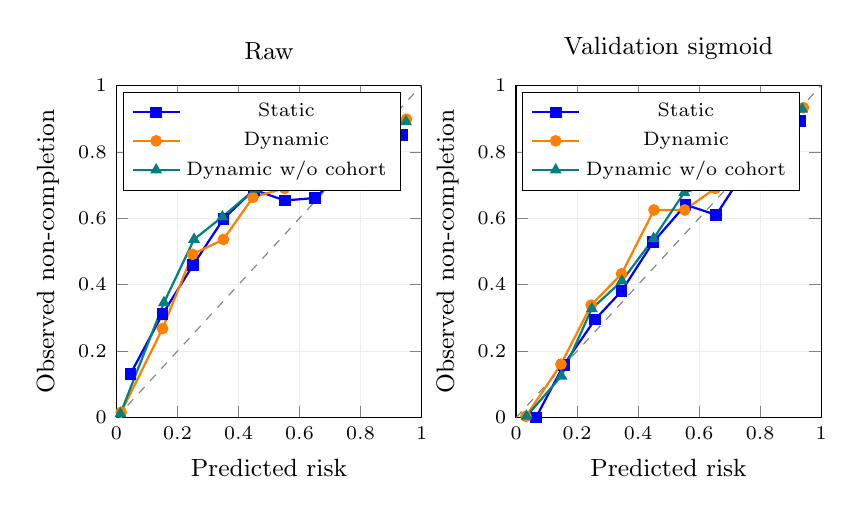
\begin{tikzpicture}
\begin{groupplot}[group style={group size=2 by 1,horizontal sep=1.2cm},width=0.45\textwidth,height=5.8cm,xmin=0,xmax=1,ymin=0,ymax=1,xlabel={Predicted risk},ylabel={Observed non-completion},tick label style={font=\scriptsize},label style={font=\small},title style={font=\small},legend style={font=\scriptsize,at={(0.02,0.98)},anchor=north west},grid=major,grid style={gray!15}]
\nextgroupplot[title={Raw}]
\addplot[gray,dashed,forget plot] coordinates {(0,0) (1,1)};
\addplot[color=blue,mark=square*,mark size=1.7pt,thick] coordinates {(0.04609813,0.13186813) (0.15061372,0.31094527) (0.25073423,0.45862069) (0.35054220,0.59807074) (0.45019656,0.68586387) (0.55207630,0.65352113) (0.65124504,0.66115702) (0.74421476,0.74338624) (0.84899045,0.83276451) (0.93797254,0.85161290)};
\addlegendentry{Static}
\addplot[color=orange,mark=*,mark size=1.7pt,thick] coordinates {(0.01538932,0.01618497) (0.15102918,0.26804124) (0.24921732,0.49152542) (0.35068032,0.53642384) (0.44745683,0.66310160) (0.55119546,0.69026549) (0.65288707,0.76900585) (0.74973011,0.88174807) (0.85537990,0.88290398) (0.95050280,0.89816701)};
\addlegendentry{Dynamic}
\addplot[color=teal,mark=triangle*,mark size=1.7pt,thick] coordinates {(0.01291693,0.01162791) (0.15578708,0.34615385) (0.25437055,0.53658537) (0.34726714,0.60427807) (0.45407259,0.68750000) (0.55463594,0.79615385) (0.65010907,0.79885057) (0.75273400,0.84097035) (0.85004056,0.89690722) (0.94911295,0.89058524)};
\addlegendentry{Dynamic w/o cohort}
\nextgroupplot[title={Validation sigmoid}]
\addplot[gray,dashed,forget plot] coordinates {(0,0) (1,1)};
\addplot[color=blue,mark=square*,mark size=1.7pt,thick] coordinates {(0.06513813,0.00000000) (0.15679251,0.15899582) (0.25870842,0.29496403) (0.34613370,0.38108108) (0.44901034,0.52789700) (0.55583957,0.64062500) (0.65591471,0.61004785) (0.75175531,0.74560000) (0.84672904,0.79615385) (0.93142627,0.89285714)};
\addlegendentry{Static}
\addplot[color=orange,mark=*,mark size=1.7pt,thick] coordinates {(0.03241866,0.00382166) (0.14716271,0.16037736) (0.24620120,0.33846154) (0.34585696,0.43269231) (0.45225166,0.62500000) (0.55276624,0.62500000) (0.65287782,0.69014085) (0.75612411,0.77384196) (0.85567534,0.85276074) (0.94202709,0.93292683)};
\addlegendentry{Dynamic}
\addplot[color=teal,mark=triangle*,mark size=1.7pt,thick] coordinates {(0.03424465,0.00390625) (0.14885192,0.12500000) (0.24830719,0.32773109) (0.34706056,0.41121495) (0.45078301,0.53906250) (0.55143090,0.67777778) (0.64792567,0.70562771) (0.75583314,0.78820375) (0.85265053,0.85028249) (0.93759853,0.92869565)};
\addlegendentry{Dynamic w/o cohort}
\end{groupplot}
\end{tikzpicture}
\caption{temporal reliability at the midpoint. Ten fixed bins; bin counts and project-specific diagnostics are retained in the artifacts.}
\label{fig:calibration-temporal}
\end{figure}


% Source: figures/fig_calibration_cross_project.tex
\begin{figure}[htbp]
\centering
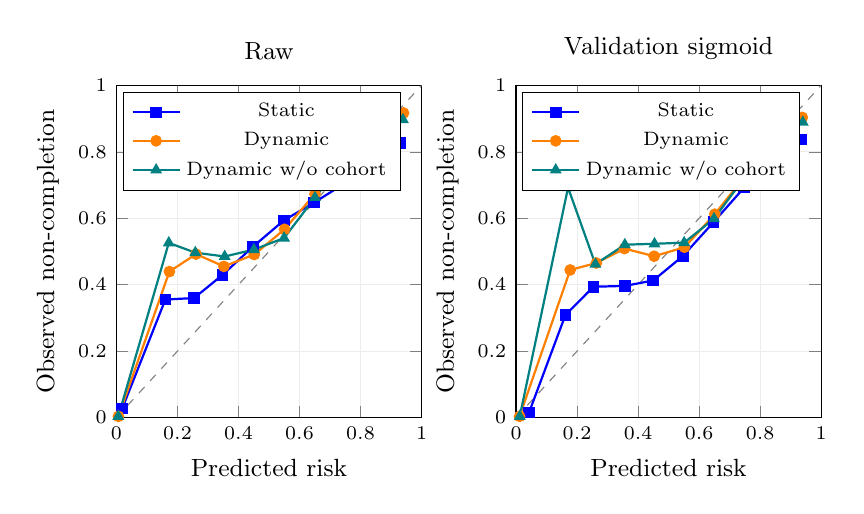
\begin{tikzpicture}
\begin{groupplot}[group style={group size=2 by 1,horizontal sep=1.2cm},width=0.45\textwidth,height=5.8cm,xmin=0,xmax=1,ymin=0,ymax=1,xlabel={Predicted risk},ylabel={Observed non-completion},tick label style={font=\scriptsize},label style={font=\small},title style={font=\small},legend style={font=\scriptsize,at={(0.02,0.98)},anchor=north west},grid=major,grid style={gray!15}]
\nextgroupplot[title={Raw}]
\addplot[gray,dashed,forget plot] coordinates {(0,0) (1,1)};
\addplot[color=blue,mark=square*,mark size=1.7pt,thick] coordinates {(0.01890877,0.02740799) (0.16033951,0.35536603) (0.25448608,0.35986267) (0.34785007,0.42959808) (0.44677685,0.51409245) (0.54885152,0.59365994) (0.64756421,0.64709596) (0.74720887,0.70462046) (0.84759645,0.73764706) (0.93013874,0.82638889)};
\addlegendentry{Static}
\addplot[color=orange,mark=*,mark size=1.7pt,thick] coordinates {(0.00661839,0.00355556) (0.17357594,0.43956044) (0.26081581,0.49218750) (0.35218861,0.45501730) (0.45173252,0.49086162) (0.55096351,0.56684492) (0.65070028,0.67338936) (0.75287441,0.76317016) (0.84795129,0.84817903) (0.94084487,0.91702742)};
\addlegendentry{Dynamic}
\addplot[color=teal,mark=triangle*,mark size=1.7pt,thick] coordinates {(0.00605578,0.00373267) (0.17155858,0.52592593) (0.25836564,0.49651568) (0.35474647,0.48498233) (0.45069916,0.50576806) (0.54935215,0.54049080) (0.65069581,0.66247265) (0.75217883,0.78111401) (0.84695536,0.85274302) (0.93896785,0.89665211)};
\addlegendentry{Dynamic w/o cohort}
\nextgroupplot[title={Validation sigmoid}]
\addplot[gray,dashed,forget plot] coordinates {(0,0) (1,1)};
\addplot[color=blue,mark=square*,mark size=1.7pt,thick] coordinates {(0.04279749,0.01567944) (0.16186320,0.30885529) (0.25392985,0.39384615) (0.35682598,0.39641358) (0.44974846,0.41273049) (0.54677188,0.48628885) (0.64769071,0.58871662) (0.74734091,0.69210664) (0.84508854,0.75917215) (0.93451898,0.83665339)};
\addlegendentry{Static}
\addplot[color=orange,mark=*,mark size=1.7pt,thick] coordinates {(0.01165470,0.00373333) (0.17747416,0.44444444) (0.26328192,0.46534653) (0.35537258,0.50877193) (0.45254953,0.48582375) (0.55214484,0.51277481) (0.65143320,0.61243781) (0.75266374,0.72972973) (0.84861775,0.83135301) (0.93821561,0.90363636)};
\addlegendentry{Dynamic}
\addplot[color=teal,mark=triangle*,mark size=1.7pt,thick] coordinates {(0.01219455,0.00373267) (0.17050783,0.69230769) (0.25999370,0.46175637) (0.35661476,0.52047556) (0.45387311,0.52317881) (0.55095937,0.52657725) (0.64879153,0.59865005) (0.75225861,0.72671622) (0.84628674,0.84373832) (0.93990489,0.88904204)};
\addlegendentry{Dynamic w/o cohort}
\end{groupplot}
\end{tikzpicture}
\caption{cross-project reliability at the midpoint. Ten fixed bins; bin counts and project-specific diagnostics are retained in the artifacts.}
\label{fig:calibration-cross-project}
\end{figure}


\subsection{Strong baselines and cumulative policies limit the deployment argument}\label{strong-baselines-and-cumulative-policies-limit-the-deployment-argument}

The fixed execution-state rule attains temporal recall of 51.23\%, compared with 53.36\% for dynamic CatBoost. The exploratory paired difference is 2.13 points (CI: -0.33--4.60), providing insufficient evidence of a temporal recall advantage over this rule. This does not establish equivalence. Cross-project project-macro gain over the rule is 3.83 points (CI: 2.10--5.73), also exploratory. Dynamic CatBoost has higher project-macro AP than the rule: 0.8128 versus 0.7517 temporal and 0.8035 versus 0.6537 cross-project.

Removing cohort context slightly increases temporal recall. The full dynamic model minus this ablation gives -0.87 points (CI: -2.26--0.29); its cross-project difference is +0.72 points (CI: 0.05--1.42). These exploratory results do not justify claiming consistent benefits from aggregate cohort features.

For cumulative alert replay, dynamic temporal recall is 51.56\%, sprint-macro precision is 77.67\%, and mean true-alert lead time is 8.30 days. The paired recall gain over the static-ranking cumulative policy is 1.30 points (CI: -0.46--3.21), inconclusive. Cross-project gain is 1.88 points (CI: 0.60--3.14), exploratory. Earlier warnings therefore do not automatically imply a stronger advantage for the learned dynamic ranker. Lead time concerns detected positives only and cannot describe how early all non-completions were identified.

% Source: sections/07_discussion.tex
\section{Discussion}\label{discussion}

The primary experiment supports using recorded execution history rather than relying solely on conservatively reconstructed start-time information. However, the operational conclusion is narrower than ``machine learning reliably predicts sprint failure.'' The outcome is a tracker-state proxy, and much of the full-cohort advantage is associated with current completion state. Descriptive CatBoost importance assigns \texttt{dynamic\_\allowbreak{}is\_\allowbreak{}done} mean importance of 27.41\% temporal and 56.44\% cross-project, with \texttt{dynamic\_\allowbreak{}status} contributing 15.58\% and 13.90\%. These correlated feature importances are not causal explanations.

The open-only comparison suggests a smaller remaining gain. It motivates future research on prioritizing ongoing work rather than allowing easy already-completed negatives to dominate a general risk score. A stronger future comparison should combine open-only eligibility with explicitly fixed integer capacity; the present separate sensitivity analyses do not establish performance under that combined setting.

Capacity should be expressed operationally. A team may handle one alert in a two-issue cohort, but such a policy must be described as one alert rather than a strict 20\% allocation. Across organizations, shared handling capacity or capacity carried across sprints may be preferable to independently rounding a percentage in every small cohort. Optimizing such allocation is future work, not a proven property of the replay policy used here.

Calibration also needs a deployment-specific validation window. The favorable temporal result and unfavorable cross-project Brier result do not support a universal probability threshold or universal benefit from sigmoid recalibration. Model versions, data completeness, eligible populations, realized capacity, and alert outcomes should be logged in a pilot.

Finally, learned models should retain strong simple comparators. The inconclusive temporal rule comparison and cumulative-policy contrast limit claims that a more complex ranker is necessary. A prospective pilot can compare a rule and a learned model under the same capacity while measuring handling cost and later delivery outcomes. The present study cannot establish which system changes practitioner behavior or reduces non-completion.

% Source: sections/08_validity.tex
\section{Threats to Validity}\label{threats-to-validity}

\textbf{Construct validity.} Terminal names are not original Jira status-category metadata, and no human workflow ground truth or inter-rater agreement is available. A recorded terminal state may include administrative closure rather than delivered functionality. Archived Start\_Date and End\_Date have no historical revision log in this dataset; their availability and stability at sprint start are assumptions. Project ownership is likewise snapshot metadata. These limitations prevent an unconditional claim of historically faithful business-commitment prediction.

\textbf{Selection and missingness.} Only 77.04\% of reconstructed commitments receive an assessable outcome, and eligibility further restricts evaluation to 14 projects. Unassessable outcomes may systematically differ from retained outcomes. Retrospective inconsistency filtering also uses later quality evidence. Static attributes missing timestamped support are not backfilled, potentially weakening the start-time comparator relative to complete real-world initial issue data. The experiment measures the value of the reconstructed information sets, not all information a team originally possessed.

\textbf{Internal validity.} We audit event prefixes, freeze partitions, purge unavailable endpoint labels, and keep preprocessing and recalibration outside test fitting. These measures do not establish complete changelog capture or detect every incorrectly timestamped record. Adding dynamic variables changes representation dimension as well as observations; the zero-percent control helps expose, but cannot eliminate, fitting effects. One fixed CatBoost configuration and one seed do not establish algorithmic optimality.

\textbf{Statistical conclusion validity.} Sprint pairing preserves the primary comparison but does not eliminate dependence from recurring issues, overlapping work, or repositories shared across projects. Cross-project bootstrap has only 14 project units and overlapping training populations across folds. Supplementary comparisons are not multiplicity-adjusted and are not confirmatory replacements for H1. Calibration plots have bins of unequal sample size; small-bin apparent deviations need cautious interpretation.

\textbf{External validity.} The sample concerns historical open-source Jira data rather than current enterprise deployment. Project holdout is not organization holdout, and cross-project evaluation is not a global time-cutoff experiment. Evaluated alert cohorts contain only assessable outcomes, whereas an online system would not know outcome assessability in advance. Offline recall, precision, and lead time do not demonstrate causal benefit from alert intervention.

% Source: sections/09_reproducibility.tex
\section{Reproducibility and Ethical Considerations}\label{reproducibility-and-ethical-considerations}

The implementation uses PostgreSQL for the imported TAWOS source and Python modules for reconstruction, fitting, evaluation, and analysis. FastAPI and Docker Compose provide the surrounding local data-access stack; no production Agentick integration or practitioner pilot was conducted. The experimental runtime is Python 3.12.10, CatBoost 1.2.10, scikit-learn 1.9.1, pandas 3.0.6, and NumPy 2.5.3, with complete installed-version manifests retained.

The local record includes the pre-fit protocol/configuration/splits, inclusion and exclusion tables, feature dictionary, sampled SQL audits, model and calibration artifacts, test predictions, and per-sprint/project result tables. Six methods over four landmarks, fourteen folds, and two evaluation settings yield 672 method--landmark--fold artifact triplets; this includes deterministic baselines and should not be interpreted as 672 independently trained learning algorithms. Every triplet was checked against the frozen test cohort and sampled re-inference. Fourteen automated tests cover key replay, split, metric, and budget invariants. Tests support implementation correctness, not the external business validity of labels.

The underlying dataset is provided by its original authors \cite{tawosi2022tawos,tawosv11}. Its research-use terms and Apache 2.0 license are recorded in the data card. We do not use contributor identity as a feature or attempt re-identification. The artifact package currently resides in this local project and Git history; \textbf{no public repository, permanent artifact DOI, or independent reproduction is claimed}. The exact commands and paths are provided in Appendix A. Publication would require an appropriately prepared public package consistent with source terms.

% Source: sections/10_conclusion.tex
\section{Conclusion}\label{conclusion}

Recorded execution histories improve midpoint identification of recorded sprint non-completion over start-time inputs in the assessed TAWOS population. The primary temporal gain is 8.90 percentage points under an upward-rounded nominal 20\% alert policy, and the secondary project-transfer gain is 9.96 points. These findings require important qualifications: open-only gain is smaller, integer rounding materially changes realized capacity, a simple execution-state rule is competitive on temporal recall, and recalibration does not universally improve transferred probability quality. The evidence supports research on explicit capacity and ongoing-work eligibility, rather than unconditional deployment or novelty claims about the learner. Prospective evaluation with historical deadline metadata, verified workflow semantics, and practitioner intervention outcomes remains necessary.

% Source: bibliography.tex
% Generated from references.bib; edit that file, then rebuild.
\begin{thebibliography}{9}
\bibitem{tawosi2022tawos} Vali Tawosi; Afnan Al-Subaihin; Rebecca Moussa; Federica Sarro. \emph{A versatile dataset of agile open source software projects}. Proceedings of the 19th international conference on mining software repositories. pp.~707--711. 2022. \url{https://doi.org/10.1145/3524842.3528029}.
\bibitem{tawosv11} SOLAR Group. \emph{The TAWOS dataset, version 1.1}. 2022. \url{https://doi.org/10.5522/04/21308124}. Repository and terms accessed 2026-10-08; source snapshot pinned by checksum.
\bibitem{tu2018careful} Feifei Tu; Jiaxin Zhu; Qimu Zheng; Minghui Zhou. \emph{Be careful of when: An empirical study on time-related misuse of issue tracking data}. Proceedings of the ACM joint meeting on european software engineering conference and symposium on the foundations of software engineering. 2018. \url{https://doi.org/10.1145/3236024.3236054}.
\bibitem{teinemaa2019outcome} Irene Teinemaa; Marlon Dumas; Marcello La Rosa; Fabrizio Maria Maggi. \emph{Outcome-oriented predictive process monitoring: Review and benchmark}. ACM Transactions on Knowledge Discovery from Data. Vol.~13(2). 2019. \url{https://doi.org/10.1145/3301300}.
\bibitem{prokhorenkova2018catboost} Liudmila Prokhorenkova; Gleb Gusev; Aleksandr Vorobev; Anna Veronika Dorogush; Andrey Gulin. \emph{CatBoost: Unbiased boosting with categorical features}. Advances in neural information processing systems. Vol.~31. 2018. \url{https://proceedings.neurips.cc/paper_files/paper/2018/hash/14491b756b3a51daac41c24863285549-Abstract.html}.
\bibitem{bui2025agents} Thanh-Long Bui; Hoa Khanh Dam; Rashina Hoda. \emph{An LLM-based multi-agent framework for agile effort estimation}. 2025. \url{https://arxiv.org/abs/2509.14483}.
\bibitem{sklearncalibration} scikit-learn developers. \emph{Probability calibration}. \url{https://scikit-learn.org/stable/modules/calibration.html}. Documentation accessed 2026-10-08; experiments use scikit-learn 1.9.1.
\end{thebibliography}

\appendix
% Source: sections/11_artifact_map.tex
\section{Artifact Map}\label{artifact-map}

{\def\LTcaptype{table}
% Source: tables/artifact_map.tex
\begin{longtable}{@{}>{\raggedright\arraybackslash}p{0.28\linewidth}>{\raggedright\arraybackslash}p{0.66\linewidth}@{}}
\caption{Local artifact map. Paths are relative to the repository root.}\label{tab:artifact_map}\\
\toprule
Evidence & Local artifact \\
\midrule
Frozen design & Protocol v1; \texttt{artifacts/\allowbreak{}protocol/\allowbreak{}config.json}, \texttt{lock.json} \\
Source and population & Data card; \texttt{artifacts/\allowbreak{}audit/\allowbreak{}}, \texttt{artifacts/\allowbreak{}dataset/\allowbreak{}} \\
Temporal/project partitions & \texttt{artifacts/\allowbreak{}protocol/\allowbreak{}temporal\_\allowbreak{}split\_\allowbreak{}manifest.csv}, \texttt{cross\_\allowbreak{}project\_\allowbreak{}split\_\allowbreak{}manifest.csv} \\
Replay and feature audit & \texttt{research/\allowbreak{}replay.py}, \texttt{research/\allowbreak{}build.py}; \texttt{artifacts/\allowbreak{}validation/\allowbreak{}feature\_\allowbreak{}dictionary.csv}, \texttt{sql\_\allowbreak{}sample\_\allowbreak{}audit.csv} \\
Fitting and raw/recalibrated predictions & \texttt{research/\allowbreak{}train.py}; \texttt{artifacts/\allowbreak{}models/\allowbreak{}}, \texttt{artifacts/\allowbreak{}predictions/\allowbreak{}}, \texttt{artifacts/\allowbreak{}runs/\allowbreak{}} \\
Primary/secondary quantitative results & \texttt{artifacts/\allowbreak{}results/\allowbreak{}paired\_\allowbreak{}comparisons.csv}, \texttt{alert\_\allowbreak{}budget\_\allowbreak{}metrics.csv}, \texttt{probability\_\allowbreak{}metrics.csv}, \texttt{sensitivity\_\allowbreak{}metrics.csv} \\
Explicit post-hoc comparisons & \texttt{artifacts/\allowbreak{}results/\allowbreak{}posthoc\_\allowbreak{}comparisons.csv}, \texttt{budget\_\allowbreak{}population\_\allowbreak{}diagnostics.json} \\
Sequential policy & \texttt{artifacts/\allowbreak{}results/\allowbreak{}sequential\_\allowbreak{}sprint\_\allowbreak{}metrics.csv}, \texttt{sequential\_\allowbreak{}alert\_\allowbreak{}log.csv} \\
Runtime and integrity & \texttt{artifacts/\allowbreak{}environment/\allowbreak{}}; \texttt{artifacts/\allowbreak{}validation/\allowbreak{}prediction\_\allowbreak{}validation.json}, \texttt{completion\_\allowbreak{}audit.json} \\
Commands & Reproduction guide \\
\bottomrule
\end{longtable}

}

Large source/model/prediction files are retained locally and excluded from Git. A clone of tracked files alone is not a complete copy of the executable data package.

\end{document}
